\section{Формальная верификация программ}

В этой главе мы несколько подробнее обсудим некоторые методы формальной верификации программ. Мы увидим, на что они опираются, в каких предположениях действуют и какова их выразительная сила. Кроме того, мы обсудим, где лежат корни идеи формальной верификации программ.

\subsection{Историческая справка}

Соггласно \cite{omodeo2017martin}, еще в пятидесятых годах прошлого века Мартином Девисом(англ. Martin Davis) было представлено первое формальное доказательство, полученное автоматически -- доказательство того, что произведение двух четных чисел четно в арифметике Пресбургера. Спустя короткое время, уже в конце шестидесятых, начали появляться первые автоматические доказатели теорем, которые использовались для верификации программ, написанных на таких языках, как \textbf{Pascal} и \textbf{Ada}.

Еще позже, в 1972 году, Робином Милнером(англ. Robin Milner) была создана система проверки доказательств \textbf{LCF}(Logic for Computable Functions), которая положила начало современным системам автоматического доказательства теорем, таким как \textbf{HOL} или \textbf{Coq}. На текущий момент, Coq является одним из самых популярных инструментов формальной верификации и автоматического доказательства теорем.

У доказателей теорем есть один недостаток, который заключается в том, что если некоторое утверждение \textbf{не} является теоремой в некоторой логике, то доказатель ничего не сможет вам об этом сказать. Иначе говоря, доказатели теорем годятся только в случае, если мы заведомо знаем, что наше утверждение является истинным и хотим получить формальное доказательство этого факта.

Для верификации конкурентных(многопоточных) программ широко используются другие методы, например проверка моделей. Их история начинается в восьмидесятых годах с работ Аллена Эмерсона и Эдмунда Кларка(англ. E. Allen Emerson и Edmund M. Clarke) о применении в этой области темпоральной логики, например -- \cite{Clarke:1981:DSS:648063.747438}. Важной особенностью именно этой работы было то, что их алгоритм был пригоден для работы с частичными спецификациями и мог приводить контрпримеры для свойств, которые не мог доказать.

Недостатком проверки моделей является следующий момент. Так как их применяют для анализа систем, которые находятся в некотором состоянии, то размер пространства состояний может экспоненциально зависеть от сложности программы. Следовательно задача анализа такой системы может быть затруднительна с вычислительной точки зрения. Для борьбы с этой проблемой зачастую используют всевозможные методы понижения размерности либо решают эту задачу приближенными методами.

Если оторваться от контекста индустрии разработки ПО, то принцип верификации был выдвинут еще в тридцатых годах. Студенты и преподаватели кафедры философии индуктивных наук Венского университета собирали семинар, более известный как Венский Кружок. Именно там под влиянием идей еще Эрнста Маха(нем. Ernst Mach), выдвинувшего мысль о том, что <<суждения, которые не могут быть ни проверены, ни отвергнуты не имеют отношения к науке>> -- цитата по \cite{wiki:mach} был сформулирован принцип верификационизма, утверждавший о том, что к реальному миру имеют отношения лишь те суждения, которые можно проверить экспериментом.

\subsection{Системы типов и \texorpdfstring{$\lambda$}{лямбда}-исчисление}

В основе систем автоматического доказательства теорем, как правило, лежит вычислительнный формализм, известный как $\lambda$-исчисление. Это формальная система, придуманная в 30-ых годах прошлого века Алонзо Черчём(англ. Alonso Church)~\cite{church1936unsolvable} с целью анализа и формализации понятия вычислимости. В 60-ых годах Питером Ландином(англ. Peter Landin) была опубликована работа~\cite{landin1964mechanical}, в которой выдвигалась идея о том, что $\lambda$-исчисление может использоваться для моделирования различных выражений в языках программирования того времени, что в дальнейшем привело к развитию языков в стиле \textbf{ML}. С тех пор идеи $\lambda$-исчисления широко используются в мире функционального программирования.

Формально, $\lambda$-термы определяются индуктивно, следующим образом:

\begin{enumerate}
  \item Если $x$ -- переменная, то $x$ -- $\lambda$-терм.
  \item Если $M$ и $N$ -- $\lambda$-термы, то $M\ N$ -- тоже $\lambda$-терм.
  \item Если $x$ -- переменная, а $M$ -- $\lambda$-терм, то $\lambda x.M$ -- тоже $\lambda$-терм.
\end{enumerate}

Изначально, в $\lambda$-исчислении не вводилось никаких правил типизации(встречается термин <<бестиповое>> или <<чистое>> $\lambda$-исчисление, англ. untyped $\lambda$-calculus), однако в дальнейшем появилось множество типизированных вариаций. Хенком Барендрегтом(нидерл. Hendrik Pieter Barendregt) в~\cite{barendregt1993lambda} описан так называемый $\lambda$-куб, который наглядно классифицирует восемь различных систем типизации лямбда-исчисления.

\begin{figure}[H]
  \centering
  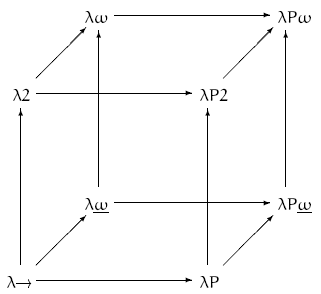
\includegraphics[width=0.5\textwidth]{img/Lambda_cube.png}
  \caption{Лямбда-куб}
\end{figure}

База куба -- просто типизированное $\lambda$-исчисление($\lambda{\to}$), в котором термы могут зависеть только от термов. Три оси соответствуют расширениям, комбинации которых позволяют получить остальные системы типов:

\begin{enumerate}
  \item Термы, которые зависят от типов -- система $\lambda2$ или \textbf{System F}
  \item Типы, которые зависят от типов -- система $\lambda \underline{\omega}$(операторы над типами)
  \item Типы, которые зависят от термов -- система $\lambda P$(зависимые типы)
\end{enumerate}

Нам не очень сейчас важно, каким образом устроены конкретные системы типов. Вместо этого, мы обсудим, какое отношение они имеют к доказателям теорем.

Соответствие Карри-Говарда~\cite{howard1980formulae} устанавливает прямую связь между логикой и теорией типов. Логической связке соответствует конструкция в теории типов, а логическому утверждению -- тип. Доказательству того факта, что утверждение истинно, соответствует тогда доказательство того факта, что соответствующий этому утверждению тип населен. То есть для доказательства утверждений мы можем писать программы на языке $\lambda$-исчисления, имеющие требуемый тип, тогда при проверке типов специальный компонент проверит, является ли наше доказательство корректным по отношению к исходному утверждению.

Незамедлительно становится ясно, что чем больше конструкций в своем распоряжений мы имеем в системе типов, тем более большой класс утверждений мы можем доказывать. Например, система автоматического доказательства теорем \textbf{Coq} основана на так называемом исчислении конструкций, соответствующему вершине $\lambda{}P{}\omega$ лямбда-куба.

Кроме этого, становится ясно, какие ограничения есть у доказателей теорем. Поскольку мы хотим выводить и проверять, является ли доказательство корректным, то нам хочется, что бы проверка типов в нашем языке всегда завершалась за конечное число шагов -- иначе говоря, была разрешимой. На этапе проверки типов может происходить вычисление значений функций, которые мы определили в нашем языке. Как следствие, от функций, которые мы определяем в нашей теории требуется, что бы они были определены для всех значений входных параметров(то есть быть тотальными).

\subsection{Темпоральная логика}

Теоретической основой для проверки моделей является, в частности, так называемая темпоральная логика. От более или менее привычной нам классической или интуиционистской логики она отличается аппарата, позволяющего рассуждать о высказываниях во временн\'{о}м аспекте. Еще во времена Аристотеля, стало понятно, что некоторым высказываниям нельзя приписать определенное истинностное значение в текущий момент времени, например <<завтра флоты столкнутся в битве>>. Эту проблему изучали философы мегарской школы, которые, в частности, ввели подобие темпоральных операторов <<возможно>> и <<необходимо>>.

В средние века темпоральной логикой занимался Уильям Оккамский(англ. William of Ockham), который выдвинул идею о том, что человек не знает истинностное значение высказываний, относящихся к будущему по той причине, что это значение известно только лишь богу. Однако, по его мнению, человек волен выбирать между различными возможными сценариями развития будущего. Современная же темпоральная логика появилась в пятидесятых годах прошлого столетия в работах Артура Приора(англ. Arthur Prior), например в \cite{prior1958time}.

Интуитивно, темпоральную логику можно представить, как формальную систему, в которой кроме обычных логических связок(конъюнкция, дизъюнкция, отрицание и импликация) есть еще и так называемые модальные связки, которые определяются следующим образом:

Бинарные:
\begin{enumerate}
  \item \textbf{Until}
  \item \textbf{Release}
\end{enumerate}

Унарные:
\begin{enumerate}
  \item \textbf{Next}
  \item \textbf{Future}
  \item \textbf{Globally}
  \item \textbf{All}
  \item \textbf{Exists}
\end{enumerate}

